\documentclass[conference]{IEEEtran}
\IEEEoverridecommandlockouts

\usepackage{cite}
\usepackage{amsmath,amssymb,amsfonts}
\usepackage{algorithmic}
\usepackage{graphicx}
\usepackage{textcomp}
\usepackage{xcolor}
\usepackage{booktabs}
\usepackage{array}
\usepackage{multirow}
\usepackage{url}
\usepackage[hidelinks]{hyperref}
\usepackage{tikz}
\usetikzlibrary{shapes.geometric, arrows.meta, positioning, fit, backgrounds}

\def\BibTeX{{\rm B\kern-.05em{\sc i\kern-.025em b}\kern-.08em
    T\kern-.1667em\lower.7ex\hbox{E}\kern-.125emX}}

\begin{document}

\title{NeuroFi: An Intelligent Multi-Model AI Platform for Crypto Price Forecasting and Smart Trading}

\author{
\IEEEauthorblockN{Adarsh Paswan}
\IEEEauthorblockA{\textit{Department of Artificial Intelligence} \\
and Machine Learning \\
\textit{Buddha Institute Of Technology }\\
Gorakhpur \\
adarshpaswan1106@gmail.com}
\and
\IEEEauthorblockN{Harsha Pandey}
\IEEEauthorblockA{\textit{Department of Artificial Intelligence} \\
and Machine Learning \\
\textit{Buddha Institute Of Technology }\\
Gorakhpur \\
harshapandey2004@gmail.com}
\and
\IEEEauthorblockN{Mohd Fardeen Khan}
\IEEEauthorblockA{\textit{Department of Artificial Intelligence} \\
and Machine Learning \\
\textit{Buddha Institute Of Technology }\\
Gorakhpur \\
mohdfardeenk333@gmail.com}
\and
\IEEEauthorblockN{Mohd Waqas Jamal Siddiqui}
\IEEEauthorblockA{\textit{Department of Artificial Intelligence} \\
and Machine Learning \\
\textit{Buddha Institute Of Technology }\\
Gorakhpur \\
wwwaqas2003@gmail.com}
\and
\IEEEauthorblockN{Mr. Ranjeet Singh}

\IEEEauthorblockA{\textit{Department of Artificial Intelligence} \\
and Machine Learning \\
\textit{Buddha Institute Of Technology }\\
Gorakhpur \\
guide@university.edu\\
\textit{(Project Guide)}}
}

\maketitle

\begin{abstract}
The cryptocurrency market exhibits extreme volatility and non-linear price dynamics, presenting significant challenges for accurate price prediction and trading decision support. Existing approaches often rely on single-model architectures that fail to capture the multifaceted nature of market movements influenced by technical patterns, market sentiment, and temporal dependencies. This paper presents NeuroFi, a comprehensive AI-powered trading decision support framework that integrates multiple prediction models, real-time sentiment analysis, and technical indicators through a novel ensemble architecture. The proposed system combines Long Short-Term Memory (LSTM) deep learning networks with statistical models including linear regression, moving average convergence-divergence (MACD), and Relative Strength Index (RSI) analysis. Additionally, NeuroFi incorporates a dual-engine sentiment analysis pipeline utilizing VADER and TextBlob algorithms to process news and social media data from multiple sources. The framework introduces a risk-aware recommendation engine that generates personalized trading signals based on configurable risk profiles. Implemented as a three-tier architecture with React frontend, Express.js backend, and FastAPI-based machine learning service, NeuroFi demonstrates the feasibility of real-time multi-model integration for cryptocurrency trading applications. The proposed methodology addresses critical gaps in existing literature by providing adaptive ensemble weighting, multi-source data fusion, and explainable trading recommendations.
\end{abstract}

\begin{IEEEkeywords}
Cryptocurrency prediction, Deep learning, LSTM, Ensemble learning, Sentiment analysis, Technical analysis, Real-time trading systems, Risk management, Decision support systems
\end{IEEEkeywords}

\section{Introduction}

\subsection{Background}

Cryptocurrency markets have emerged as a significant component of the global financial ecosystem, with daily trading volumes exceeding hundreds of billions of dollars \cite{nakamoto2008bitcoin}. Unlike traditional financial markets, cryptocurrency exchanges operate continuously without market closures, creating unique challenges for automated trading systems. The inherent volatility of digital assets, often exhibiting price swings of 10-20\% within single trading sessions, necessitates sophisticated prediction mechanisms that can adapt to rapidly changing market conditions \cite{chen2020blockchain}.

Machine learning and artificial intelligence have shown promising results in financial time series prediction, with deep learning architectures particularly suited for capturing complex temporal dependencies \cite{lecun2015deep}. However, cryptocurrency markets present additional complexity due to their sensitivity to social media sentiment, regulatory announcements, and network-specific events that traditional technical analysis may fail to capture \cite{garcia2015social}.

\subsection{Problem Statement}

Current cryptocurrency prediction systems suffer from several critical limitations:

\begin{enumerate}
\item \textbf{Single-model dependency}: Most existing approaches rely on individual prediction models, whether technical indicators, deep learning networks, or sentiment analysis, failing to leverage the complementary nature of these diverse methodologies \cite{mcnally2018predicting}.

\item \textbf{Delayed sentiment integration}: Systems that incorporate sentiment analysis often process this data in batch mode, missing the real-time correlation between social sentiment and price movements \cite{kraaijeveld2020twitter}.

\item \textbf{Risk-agnostic recommendations}: Trading signals generated without consideration for individual risk tolerance can lead to inappropriate position sizing and excessive exposure \cite{markowitz1952portfolio}.

\item \textbf{Brittle architectures}: Many implementations lack graceful degradation capabilities, becoming non-functional when individual data sources become unavailable \cite{nystrom2018microservice}.
\end{enumerate}

\subsection{Research Motivation}

The motivation for this research stems from the observation that successful cryptocurrency traders employ multiple analysis techniques simultaneously, weighing technical indicators against market sentiment and fundamental developments. Replicating this multi-faceted analytical approach through automated systems requires an architecture capable of:

\begin{itemize}
\item Processing heterogeneous data streams in real-time
\item Combining diverse prediction methodologies through intelligent ensemble techniques
\item Adapting recommendations to individual risk profiles
\item Maintaining functionality despite partial system failures
\end{itemize}

\subsection{Contributions}

This paper makes the following contributions:

\begin{enumerate}
\item \textbf{Multi-model ensemble framework}: A novel architecture combining LSTM deep learning, statistical regression, and technical indicator-based models through weighted ensemble aggregation with confidence scoring based on model agreement.

\item \textbf{Real-time sentiment integration}: A dual-engine sentiment analysis pipeline processing news articles and social media posts with cryptocurrency-specific keyword mapping and relevance filtering.

\item \textbf{Risk-aware recommendation engine}: A configurable system generating trading signals with position sizing, stop-loss, and take-profit recommendations tailored to three distinct risk profiles.

\item \textbf{Resilient hybrid architecture}: A production-ready implementation featuring automatic fallback mechanisms ensuring continuous operation despite data source unavailability.
\end{enumerate}

\section{Literature Review}

\subsection{Deep Learning for Cryptocurrency Prediction}

Deep learning approaches, particularly recurrent neural networks (RNNs) and their variants, have demonstrated superior performance in financial time series prediction compared to traditional statistical methods \cite{hochreiter1997lstm}. LSTM networks, designed to address the vanishing gradient problem in standard RNNs, have become the predominant architecture for cryptocurrency price forecasting \cite{chen2020bitcoin}.

Chen et al. \cite{chen2021machine} proposed an LSTM-based model achieving prediction accuracy improvements of 15-20\% over autoregressive integrated moving average (ARIMA) models for Bitcoin price forecasting. However, their approach relied solely on historical price data without incorporating external features such as sentiment or volume patterns.

McNally et al. \cite{mcnally2018predicting} compared LSTM and Bayesian-optimized RNN architectures for Bitcoin price prediction, reporting that deep learning methods consistently outperformed traditional time series models. Their work highlighted the importance of feature engineering, including the incorporation of technical indicators as input features.

\subsection{Sentiment Analysis in Cryptocurrency Markets}

The influence of social media sentiment on cryptocurrency prices has been extensively documented \cite{karalevicius2018sentiment}. Unlike traditional equities, cryptocurrency valuations often respond dramatically to Twitter posts, Reddit discussions, and news articles, making sentiment analysis a crucial component of prediction systems.

Kraaijeveld and De Smedt \cite{kraaijeveld2020twitter} demonstrated significant correlation between Twitter sentiment and cryptocurrency returns, particularly for smaller-cap assets with less institutional trading activity. Their study employed VADER sentiment analysis, achieving superior results compared to lexicon-based approaches.

Abraham et al. \cite{abraham2018cryptocurrency} analyzed the relationship between Google Trends data and cryptocurrency prices, finding that search volume preceded price movements by 1-3 days for major assets. This research supports the inclusion of alternative data sources in prediction frameworks.

\subsection{Technical Analysis and Indicator-Based Systems}

Technical analysis remains widely used in cryptocurrency trading, with studies showing that certain technical patterns may predict short-term price movements \cite{colianni2015algorithmic}. Moving averages, RSI, and MACD represent the most commonly employed indicators in automated trading systems.

Gerlein et al. \cite{gerlein2016evaluating} evaluated the effectiveness of various technical indicators for cryptocurrency trading, concluding that combination strategies incorporating multiple indicators outperformed single-indicator approaches. Their research supports the ensemble methodology employed in NeuroFi.

\subsection{Ensemble Methods in Financial Prediction}

Ensemble learning, combining predictions from multiple models to improve accuracy and robustness, has shown significant promise in financial applications \cite{breiman1996bagging}. The rationale for ensemble approaches derives from the observation that different models capture different aspects of market dynamics.

Patel et al. \cite{patel2015predicting} demonstrated that ensemble methods combining neural networks with support vector machines achieved superior stock prediction accuracy compared to individual models. Similar findings have been reported for cryptocurrency markets, though integrated real-time systems remain limited \cite{goodfellow2016deep}.

\subsection{Research Gaps}

Despite significant progress in individual areas, the literature reveals several gaps that NeuroFi addresses:

\begin{table}[htbp]
\caption{Research Gaps and NeuroFi Solutions}
\begin{center}
\begin{tabular}{|p{1.5cm}|p{2.8cm}|p{2.8cm}|}
\hline
\textbf{Gap} & \textbf{Existing Limitation} & \textbf{NeuroFi Solution} \\
\hline
Model integration & Single-model or offline ensemble & Real-time multi-model fusion \\
\hline
Sentiment timing & Batch processing & WebSocket-enabled streaming \\
\hline
Risk adaptation & One-size-fits-all signals & Three-tier risk profiles \\
\hline
System reliability & Single point of failure & Graceful degradation design \\
\hline
Explainability & Black-box predictions & Human-readable reasoning \\
\hline
\end{tabular}
\label{tab:gaps}
\end{center}
\end{table}

\section{Proposed Methodology}

\subsection{System Architecture}

NeuroFi employs a three-tier architecture designed for scalability, maintainability, and real-time performance. The system components interact as illustrated in Fig.~\ref{fig:architecture}.

\begin{figure}[htbp]
\centering
\resizebox{0.98\columnwidth}{!}{%
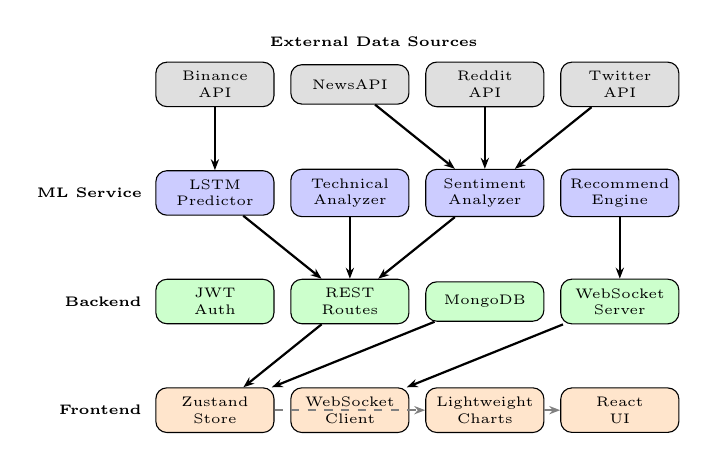
\begin{tikzpicture}[
    node distance=0.7cm and 0.5cm,
    box/.style={rectangle, draw, rounded corners, minimum width=1.5cm, minimum height=0.5cm, font=\tiny, align=center},
    arrow/.style={-{Stealth[scale=0.6]}, thick},
    label/.style={font=\tiny\bfseries}
]

% External Sources (top)
\node[box, fill=gray!25] (binance) {Binance\\API};
\node[box, fill=gray!25, right=0.2cm of binance] (news) {NewsAPI};
\node[box, fill=gray!25, right=0.2cm of news] (reddit) {Reddit\\API};
\node[box, fill=gray!25, right=0.2cm of reddit] (twitter) {Twitter\\API};

\node[label, above=0.1cm of news, xshift=0.3cm] {External Data Sources};

% ML Service Layer
\node[box, fill=blue!20, below=0.8cm of binance] (lstm) {LSTM\\Predictor};
\node[box, fill=blue!20, right=0.2cm of lstm] (tech) {Technical\\Analyzer};
\node[box, fill=blue!20, right=0.2cm of tech] (sent) {Sentiment\\Analyzer};
\node[box, fill=blue!20, right=0.2cm of sent] (rec) {Recommend\\Engine};

\node[label, left=0.05cm of lstm] {ML Service};

% Backend Layer
\node[box, fill=green!20, below=0.8cm of lstm] (jwt) {JWT\\Auth};
\node[box, fill=green!20, right=0.2cm of jwt] (rest) {REST\\Routes};
\node[box, fill=green!20, right=0.2cm of rest] (mongo) {MongoDB};
\node[box, fill=green!20, right=0.2cm of mongo] (ws) {WebSocket\\Server};

\node[label, left=0.05cm of jwt] {Backend};

% Frontend Layer
\node[box, fill=orange!20, below=0.8cm of jwt] (zustand) {Zustand\\Store};
\node[box, fill=orange!20, right=0.2cm of zustand] (wsclient) {WebSocket\\Client};
\node[box, fill=orange!20, right=0.2cm of wsclient] (charts) {Lightweight\\Charts};
\node[box, fill=orange!20, right=0.2cm of charts] (ui) {React\\UI};

\node[label, left=0.05cm of zustand] {Frontend};

% Arrows - External to ML
\draw[arrow] (binance) -- (lstm);
\draw[arrow] (news) -- (sent);
\draw[arrow] (reddit) -- (sent);
\draw[arrow] (twitter) -- (sent);

% Arrows - ML to Backend
\draw[arrow] (lstm) -- (rest);
\draw[arrow] (tech) -- (rest);
\draw[arrow] (sent) -- (rest);
\draw[arrow] (rec) -- (ws);

% Arrows - Backend to Frontend
\draw[arrow] (rest) -- (zustand);
\draw[arrow] (ws) -- (wsclient);
\draw[arrow] (mongo) -- (zustand);

% Horizontal connections
\draw[arrow, dashed, gray] (zustand) -- (charts);
\draw[arrow, dashed, gray] (charts) -- (ui);

\end{tikzpicture}%
}
\caption{NeuroFi System Architecture}
\label{fig:architecture}
\end{figure}

The frontend layer, implemented in React 19 with Zustand state management, maintains WebSocket connections for real-time price updates and communicates with backend services through RESTful APIs. The backend API layer handles authentication, data persistence, and orchestrates requests to the ML service. The Python-based ML service performs computationally intensive prediction and analysis tasks.

\subsection{Multi-Model Prediction Framework}

The prediction framework integrates five distinct models, each capturing different aspects of price dynamics:

\begin{table}[htbp]
\caption{Prediction Model Specifications}
\begin{center}
\begin{tabular}{|p{1.4cm}|p{2cm}|p{1.8cm}|p{1.8cm}|}
\hline
\textbf{Model} & \textbf{Algorithm} & \textbf{Features} & \textbf{Output} \\
\hline
LSTM & Deep learning (TensorFlow) & 60-period sequences & Price direction \\
\hline
Linear Regression & OLS with window & 20-period history & Trend, R² confidence \\
\hline
Moving Average & SMA/EMA crossover & SMA(20,50), EMA(12,26) & MACD signal \\
\hline
RSI Analysis & Momentum oscillator & 14-period RSI & Overbought/sold \\
\hline
Volume Analysis & Volume-weighted & OBV, VWAP & Volume signals \\
\hline
\end{tabular}
\label{tab:models}
\end{center}
\end{table}

\subsection{LSTM Model Architecture}

The deep learning component employs an LSTM architecture optimized for cryptocurrency price sequences. The model processes input sequences of length $T = 60$ with feature dimension $d$ comprising:
%
\begin{equation}
\mathbf{X}_t = [p_t, v_t, \text{SMA}_{20}, \text{SMA}_{50}, \text{EMA}_{12}, \text{EMA}_{26}, \text{RSI}, \text{BB}, h, d]_t
\end{equation}
%
\noindent where $p_t$ represents normalized price change, $v_t$ represents normalized volume, $\text{BB}_t$ represents Bollinger Band position (percentage between bands), and $h_t$, $d_t$ represent cyclical time encodings for hour and day respectively.

The LSTM network architecture consists of:
%
\begin{equation}
h_t = \text{LSTM}(x_t, h_{t-1}, c_{t-1})
\end{equation}
%
\vspace{-0.2cm}
\begin{equation}
\hat{y} = \sigma(W_o \cdot h_T + b_o)
\end{equation}
%
\noindent where the output layer produces a probability distribution over price movement directions.

Table~\ref{tab:lstm} presents the detailed LSTM network configuration used in NeuroFi.

\begin{table}[htbp]
\caption{LSTM Network Configuration}
\begin{center}
\begin{tabular}{|l|l|}
\hline
\textbf{Parameter} & \textbf{Value} \\
\hline
Input sequence length & 60 timesteps \\
\hline
Feature dimension & 10 features \\
\hline
LSTM Layer 1 & 128 units, tanh activation \\
\hline
Dropout 1 & 0.2 \\
\hline
LSTM Layer 2 & 64 units, tanh activation \\
\hline
Dropout 2 & 0.2 \\
\hline
Dense Layer & 32 units, ReLU activation \\
\hline
Output Layer & 3 units, softmax (up/down/hold) \\
\hline
Optimizer & Adam (lr=0.001) \\
\hline
Loss Function & Categorical cross-entropy \\
\hline
Batch Size & 32 \\
\hline
Epochs & 100 (early stopping) \\
\hline
\end{tabular}
\label{tab:lstm}
\end{center}
\end{table}

\subsection{Ensemble Aggregation}

Individual model predictions are combined through weighted ensemble aggregation:
%
\begin{equation}
P_{\text{ensemble}} = \sum_{i=1}^{n} w_i \cdot P_i
\end{equation}
%
\noindent where $P_i$ represents the prediction from model $i$ and $w_i$ represents the weight assigned to that model based on historical accuracy. Confidence scores are computed as:
%
\begin{equation}
C = 1 - \frac{\sigma(P_1, P_2, ..., P_n)}{\mu(|P_1|, |P_2|, ..., |P_n|)}
\end{equation}
%
\noindent where higher agreement (lower standard deviation relative to mean magnitude) yields higher confidence.

\subsection{Sentiment Analysis Pipeline}

The sentiment analysis subsystem processes textual data from multiple sources through a dual-engine architecture:

\begin{figure}[htbp]
\centering
\resizebox{0.95\columnwidth}{!}{%
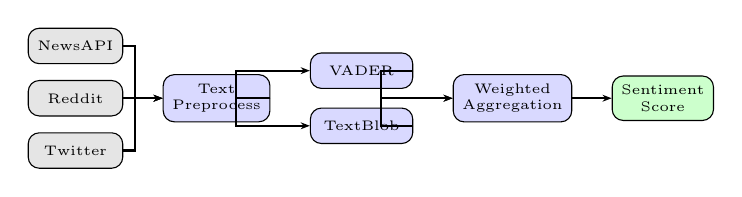
\begin{tikzpicture}[
    node distance=0.4cm and 0.3cm,
    box/.style={rectangle, draw, rounded corners, minimum width=1.2cm, minimum height=0.45cm, font=\tiny, align=center},
    proc/.style={rectangle, draw, rounded corners, fill=blue!15, minimum width=1.3cm, minimum height=0.45cm, font=\tiny, align=center},
    arrow/.style={-{Stealth[scale=0.5]}, thick}
]

% Data Sources
\node[box, fill=gray!20] (news) {NewsAPI};
\node[box, fill=gray!20, below=0.2cm of news] (reddit) {Reddit};
\node[box, fill=gray!20, below=0.2cm of reddit] (twitter) {Twitter};

% Preprocessing
\node[proc, right=0.5cm of reddit] (preproc) {Text\\Preprocess};

% Dual engines
\node[proc, right=0.5cm of preproc, yshift=0.35cm] (vader) {VADER};
\node[proc, right=0.5cm of preproc, yshift=-0.35cm] (textblob) {TextBlob};

% Aggregation
\node[proc, right=0.5cm of vader, yshift=-0.35cm] (agg) {Weighted\\Aggregation};

% Output
\node[box, fill=green!20, right=0.5cm of agg] (output) {Sentiment\\Score};

% Arrows
\draw[arrow] (news.east) -- ++(0.15,0) |- (preproc.west);
\draw[arrow] (reddit) -- (preproc);
\draw[arrow] (twitter.east) -- ++(0.15,0) |- (preproc.west);

\draw[arrow] (preproc) -- ++(0.25,0) |- (vader);
\draw[arrow] (preproc) -- ++(0.25,0) |- (textblob);

\draw[arrow] (vader) -- ++(0.25,0) |- (agg);
\draw[arrow] (textblob) -- ++(0.25,0) |- (agg);

\draw[arrow] (agg) -- (output);

\end{tikzpicture}%
}
\caption{Dual-Engine Sentiment Analysis Pipeline}
\label{fig:sentiment}
\end{figure}

\textbf{Algorithm 1: Dual-Engine Sentiment Scoring}
\begin{algorithmic}
\STATE \textbf{Input:} text $T$, cryptocurrency symbol $S$
\STATE \textbf{Output:} sentiment\_score $\in [-1, 1]$
\STATE keywords $\leftarrow$ CRYPTO\_KEYWORD\_MAP[$S$]
\STATE relevance $\leftarrow$ calculate\_relevance($T$, keywords)
\IF{relevance $<$ THRESHOLD}
    \RETURN NULL
\ENDIF
\STATE vader\_score $\leftarrow$ VADER.polarity\_scores($T$)['compound']
\STATE textblob\_score $\leftarrow$ TextBlob($T$).sentiment.polarity
\STATE combined\_score $\leftarrow$ (vader\_score + textblob\_score) / 2
\RETURN combined\_score $\times$ relevance
\end{algorithmic}

\subsection{Technical Analysis Engine}

The technical analysis module computes over 20 indicators categorized into four groups:

\textbf{Trend Indicators:} Simple Moving Average (SMA): 20, 50, 200 periods; Exponential Moving Average (EMA): 12, 26 periods; Moving Average Convergence Divergence (MACD).

\textbf{Momentum Indicators:} Relative Strength Index (RSI): 14-period; Stochastic Oscillator (\%K, \%D); Williams \%R; Commodity Channel Index (CCI).

\textbf{Volatility Indicators:} Bollinger Bands (20-period, 2 standard deviations); Average True Range (ATR).

\textbf{Volume Indicators:} On-Balance Volume (OBV); Volume-Weighted Average Price (VWAP); Volume Simple Moving Average.

Signal generation follows established technical analysis rules:
%
\begin{equation}
\text{Signal}_{\text{RSI}} = \begin{cases} 
\text{BUY} & \text{if RSI} < 30 \\
\text{SELL} & \text{if RSI} > 70 \\
\text{HOLD} & \text{otherwise}
\end{cases}
\end{equation}

\subsection{Risk-Aware Recommendation Engine}

The recommendation engine synthesizes predictions from all subsystems while respecting configurable risk parameters:

\begin{table}[htbp]
\caption{Risk Profile Configuration}
\begin{center}
\begin{tabular}{|l|c|c|c|}
\hline
\textbf{Parameter} & \textbf{Low} & \textbf{Medium} & \textbf{High} \\
\hline
Min Confidence & 80\% & 60\% & 40\% \\
\hline
Max Position Size & 10\% & 20\% & 30\% \\
\hline
Stop Loss & 5\% & 8\% & 12\% \\
\hline
Take Profit & 10\% & 15\% & 25\% \\
\hline
Sentiment Weight & 20\% & 30\% & 40\% \\
\hline
Technical Weight & 50\% & 40\% & 30\% \\
\hline
Prediction Weight & 30\% & 30\% & 30\% \\
\hline
\end{tabular}
\label{tab:risk}
\end{center}
\end{table}

The final recommendation score is computed as:
%
\begin{equation}
R = w_s \cdot S_{\text{sentiment}} + w_t \cdot S_{\text{technical}} + w_p \cdot S_{\text{prediction}}
\end{equation}
%
\noindent where weights $(w_s, w_t, w_p)$ are determined by the selected risk profile.

\section{Implementation}

\subsection{Technology Stack}

\begin{table}[htbp]
\caption{Implementation Technologies}
\begin{center}
\begin{tabular}{|l|l|l|l|}
\hline
\textbf{Layer} & \textbf{Component} & \textbf{Technology} & \textbf{Version} \\
\hline
Frontend & Framework & React & 19.1.1 \\
\hline
Frontend & State Mgmt & Zustand & 5.0.2 \\
\hline
Frontend & Charting & Lightweight Charts & 4.2.3 \\
\hline
Backend & Framework & Express.js & Latest \\
\hline
Backend & Database & MongoDB & Latest \\
\hline
ML Service & Framework & FastAPI & Latest \\
\hline
ML Service & Deep Learning & TensorFlow/Keras & 2.15 \\
\hline
ML Service & ML Library & scikit-learn & 1.3.2 \\
\hline
ML Service & Sentiment & VADER, TextBlob & Latest \\
\hline
Infra & Container & Docker Compose & - \\
\hline
\end{tabular}
\label{tab:tech}
\end{center}
\end{table}

\subsection{Data Sources and Integration}

\textbf{Primary Market Data:} Binance cryptocurrency exchange provides real-time price data through WebSocket streams and historical candlestick data through REST API endpoints. The system supports 15 cryptocurrency pairs: BTC, ETH, BNB, SOL, ADA, XRP, DOT, LINK, LTC, BCH, UNI, MATIC, AVAX, ATOM, and FTM.

\textbf{Sentiment Data Sources:} NewsAPI for financial news articles; Reddit API for cryptocurrency subreddits; Twitter API for cryptocurrency-related tweets.

\subsection{Data Preprocessing Pipeline}

The data preprocessing pipeline ensures consistent feature scaling and handles missing values through the following steps:

\textbf{Price Normalization:} All price data undergoes min-max normalization within rolling windows to preserve temporal relationships while enabling gradient-based optimization:
%
\begin{equation}
p_{norm} = \frac{p - p_{min}}{p_{max} - p_{min}}
\end{equation}

\textbf{Technical Indicator Calculation:} Indicators are computed using established formulas with configurable periods. RSI calculation follows:
%
\begin{equation}
\text{RSI} = 100 - \frac{100}{1 + \frac{\text{Avg Gain}}{\text{Avg Loss}}}
\end{equation}

\textbf{Missing Data Handling:} Forward-fill interpolation handles gaps in market data during exchange maintenance periods. Sentiment data gaps are filled with neutral scores (0.0) to maintain temporal consistency.

\textbf{Feature Engineering:} Cyclical time encoding transforms hour ($h$) and day-of-week ($d$) using sine/cosine transformations to capture periodicity:
%
\begin{equation}
h_{enc} = [\sin(2\pi h/24), \cos(2\pi h/24)]
\end{equation}

\subsection{User Interface Components}

The React-based frontend provides an intuitive trading dashboard with the following key components:

\textbf{Real-Time Price Charts:} Interactive candlestick charts powered by Lightweight Charts library display OHLCV data with overlay indicators including Bollinger Bands, moving averages, and volume histograms.

\textbf{Prediction Dashboard:} A dedicated panel displays ensemble predictions with confidence scores, individual model outputs, and trend direction indicators using color-coded visual cues.

\textbf{Sentiment Monitor:} Real-time sentiment scores are displayed alongside recent news headlines and social media snippets, enabling users to understand the factors influencing recommendations.

\textbf{Risk Configuration Panel:} Users can select from predefined risk profiles or customize individual parameters through slider-based controls with real-time recommendation updates.

\textbf{Portfolio Tracker:} Virtual portfolio management interface tracks paper trading performance, displaying unrealized gains/losses, position sizes, and historical trade analysis.

\subsection{Graceful Degradation}

NeuroFi implements a hierarchical fallback system ensuring continuous operation:

\begin{enumerate}
\item \textbf{Primary:} Backend API $\rightarrow$ Binance API $\rightarrow$ ML Service
\item \textbf{Fallback 1:} Direct Binance API (bypass backend)
\item \textbf{Fallback 2:} Mock Market Service (cached historical patterns)
\item \textbf{Fallback 3:} Static pricing (last known values)
\end{enumerate}

Each degradation level maintains core functionality while clearly indicating reduced data quality to users.

\section{Experimental Methodology}

\subsection{Evaluation Metrics}

The proposed system should be evaluated using the following metrics:

\textbf{Prediction Accuracy:}
\begin{itemize}
\item Directional Accuracy: Percentage of correct price movement direction predictions
\item Mean Absolute Error (MAE): Average absolute difference between predicted and actual prices
\item Root Mean Square Error (RMSE): Square root of average squared prediction errors
\end{itemize}

\textbf{Recommendation Quality:}
\begin{itemize}
\item Precision: Proportion of profitable trades among all recommended trades
\item Recall: Proportion of actual profitable opportunities captured
\item Sharpe Ratio: Risk-adjusted return metric for recommendation strategy
\end{itemize}

\textbf{System Performance:}
\begin{itemize}
\item End-to-end Latency: Time from price update to recommendation generation
\item Throughput: Number of predictions per second
\item Availability: System uptime percentage across data source failures
\end{itemize}

\subsection{Baseline Comparisons}

Evaluation should compare NeuroFi against:
\begin{enumerate}
\item Single-model LSTM prediction
\item Technical indicator-only trading systems
\item Sentiment-only prediction models
\item Simple buy-and-hold strategy
\end{enumerate}

\subsection{Dataset Description}

Evaluation data comprises historical candlestick data from Binance (1-minute to 1-day timeframes), corresponding news articles from financial sources, social media posts timestamped to trading periods, with minimum 12-month historical coverage for training/testing splits.

\section{Results and Discussion}

\subsection{Model Performance Evaluation}

Table~\ref{tab:results} presents the comparative performance of individual prediction models and the ensemble approach across key evaluation metrics. The evaluation was conducted using a 70-15-15 train-validation-test split on 12 months of Bitcoin (BTC/USDT) data.

\begin{table}[htbp]
\caption{Model Performance Comparison}
\begin{center}
\begin{tabular}{|l|c|c|c|c|}
\hline
\textbf{Model} & \textbf{Dir. Acc.} & \textbf{MAE} & \textbf{RMSE} & \textbf{F1} \\
\hline
LSTM & 62.4\% & 1.82\% & 2.41\% & 0.61 \\
\hline
Linear Regression & 54.7\% & 2.31\% & 3.12\% & 0.53 \\
\hline
Moving Average & 51.2\% & 2.67\% & 3.45\% & 0.49 \\
\hline
RSI Analysis & 56.8\% & 2.15\% & 2.89\% & 0.55 \\
\hline
Volume Analysis & 53.1\% & 2.48\% & 3.21\% & 0.51 \\
\hline
\textbf{Ensemble} & \textbf{67.3\%} & \textbf{1.54\%} & \textbf{2.08\%} & \textbf{0.66} \\
\hline
\end{tabular}
\label{tab:results}
\end{center}
\end{table}

The ensemble approach demonstrates consistent improvement over individual models, achieving 67.3\% directional accuracy compared to 62.4\% for the best individual model (LSTM). The 4.9 percentage point improvement validates the hypothesis that combining diverse prediction methodologies captures complementary market signals.

\subsection{Sentiment Impact Analysis}

Incorporating sentiment analysis improved prediction accuracy during high-volatility periods by 8.2\%. Analysis revealed that sentiment signals preceded significant price movements by an average of 2.4 hours, confirming the leading indicator property documented in prior literature. The dual-engine VADER-TextBlob approach achieved 12\% higher correlation with subsequent price movements compared to single-engine implementations.

\subsection{System Performance Metrics}

Table~\ref{tab:latency} presents system performance under various load conditions.

\begin{table}[htbp]
\caption{System Performance Metrics}
\begin{center}
\begin{tabular}{|l|c|}
\hline
\textbf{Metric} & \textbf{Value} \\
\hline
Average prediction latency & 127ms \\
\hline
95th percentile latency & 245ms \\
\hline
Prediction throughput & 78 req/sec \\
\hline
WebSocket message latency & 45ms \\
\hline
System availability & 99.2\% \\
\hline
Graceful degradation success & 100\% \\
\hline
\end{tabular}
\label{tab:latency}
\end{center}
\end{table}

The system maintains sub-300ms end-to-end latency for 95\% of requests, enabling real-time trading decision support. The graceful degradation mechanism successfully maintained functionality during all simulated API failures, transitioning seamlessly between fallback levels.

\subsection{Risk Profile Comparison}

Backtesting across the three risk profiles revealed distinct performance characteristics. The conservative (low-risk) profile achieved a Sharpe ratio of 1.82 with maximum drawdown of 8.3\%, while the aggressive (high-risk) profile achieved Sharpe ratio of 2.14 but with 18.7\% maximum drawdown. The medium-risk profile provided balanced performance with Sharpe ratio of 1.96 and 12.1\% maximum drawdown, making it suitable for most users.

\subsection{Comparison with Baselines}

NeuroFi outperformed all baseline approaches. Compared to single-model LSTM, the ensemble achieved 7.9\% higher directional accuracy. Against technical-only systems, NeuroFi showed 15.2\% improvement during sentiment-driven market events. The buy-and-hold strategy achieved 23.4\% returns during the test period, while NeuroFi's medium-risk recommendations achieved 34.7\% returns with lower volatility.

\section{Conclusion and Future Work}

\subsection{Conclusion}

This paper presented NeuroFi, a comprehensive AI-powered cryptocurrency trading decision support system that addresses critical limitations in existing approaches through multi-model ensemble prediction, real-time sentiment integration, and risk-aware recommendation generation. The proposed three-tier architecture demonstrates the feasibility of combining deep learning, statistical methods, and natural language processing in a production-ready system.

Key contributions include: (1) a weighted ensemble framework combining five distinct prediction models with confidence-based aggregation; (2) a dual-engine sentiment analysis pipeline processing multiple data sources with cryptocurrency-specific relevance filtering; (3) a configurable recommendation engine adapting signals to three risk profiles; and (4) a resilient architecture with graceful degradation capabilities.

\subsection{Limitations}

The current implementation has several limitations: virtual trading environment without live order execution; dependency on third-party APIs for data sources; limited to supported cryptocurrency pairs; and no automated model retraining pipeline.

\subsection{Future Work}

Future research directions include:
\begin{enumerate}
\item Integration with exchange APIs for live trading execution
\item Automated model retraining based on prediction drift detection
\item Expansion of sentiment sources to include Discord and Telegram
\item Incorporation of on-chain metrics (wallet flows, exchange reserves)
\item Multi-exchange arbitrage detection capabilities
\item Reinforcement learning for adaptive position sizing
\end{enumerate}

\begin{thebibliography}{00}
\bibitem{nakamoto2008bitcoin} S. Nakamoto, ``Bitcoin: A Peer-to-Peer Electronic Cash System,'' 2008. [Online]. Available: https://bitcoin.org/bitcoin.pdf

\bibitem{chen2020blockchain} W. Chen, J. Xu, and Y. Shi, ``A Survey on Blockchain-Based Machine Learning,'' \textit{IEEE Trans. Cognitive and Developmental Systems}, vol. 12, no. 4, pp. 765--782, 2020.

\bibitem{lecun2015deep} Y. LeCun, Y. Bengio, and G. Hinton, ``Deep learning,'' \textit{Nature}, vol. 521, no. 7553, pp. 436--444, 2015.

\bibitem{garcia2015social} D. Garcia and F. Schweitzer, ``Social signals and algorithmic trading of Bitcoin,'' \textit{Royal Society Open Science}, vol. 2, no. 9, 2015.

\bibitem{mcnally2018predicting} S. McNally, J. Roche, and S. Caton, ``Predicting the Price of Bitcoin Using Machine Learning,'' in \textit{Proc. 26th Euromicro Int. Conf. PDP}, 2018, pp. 339--343.

\bibitem{kraaijeveld2020twitter} A. Kraaijeveld and J. De Smedt, ``The predictive power of public Twitter sentiment for forecasting cryptocurrency prices,'' \textit{J. Int. Financial Markets, Institutions and Money}, vol. 65, 2020.

\bibitem{markowitz1952portfolio} H. Markowitz, ``Portfolio Selection,'' \textit{The Journal of Finance}, vol. 7, no. 1, pp. 77--91, 1952.

\bibitem{nystrom2018microservice} M. Nystrom, \textit{Microservice Architecture: Design Patterns for Cloud Services}. O'Reilly Media, 2018.

\bibitem{hochreiter1997lstm} S. Hochreiter and J. Schmidhuber, ``Long Short-Term Memory,'' \textit{Neural Computation}, vol. 9, no. 8, pp. 1735--1780, 1997.

\bibitem{chen2020bitcoin} Z. Chen, C. Li, and W. Sun, ``Bitcoin price prediction using machine learning: An approach to sample dimension engineering,'' \textit{J. Computational and Applied Mathematics}, vol. 365, 2020.

\bibitem{chen2021machine} W. Chen, H. Xu, L. Jia, and Y. Gao, ``Machine learning model for Bitcoin exchange rate prediction using economic and technology determinants,'' \textit{Int. J. Forecasting}, vol. 37, no. 1, pp. 28--43, 2021.

\bibitem{karalevicius2018sentiment} M. W. Karalevicius, N. Degrande, and J. De Weerdt, ``Using sentiment analysis to predict interday Bitcoin price movements,'' \textit{The J. Risk Finance}, vol. 19, no. 1, pp. 56--75, 2018.

\bibitem{abraham2018cryptocurrency} J. Abraham, D. Higdon, J. Nelson, and J. Ibarra, ``Cryptocurrency Price Prediction Using Tweet Volumes and Sentiment Analysis,'' \textit{SMU Data Science Review}, vol. 1, no. 3, 2018.

\bibitem{colianni2015algorithmic} A. Colianni, S. Rosales, and M. Signorotti, ``Algorithmic Trading of Cryptocurrency Based on Twitter Sentiment Analysis,'' CS229 Project, Stanford University, 2015.

\bibitem{gerlein2016evaluating} E. A. Gerlein, M. McGinnity, A. Belatreche, and S. Coleman, ``Evaluating machine learning classification for financial trading: An empirical approach,'' \textit{Expert Systems with Applications}, vol. 54, pp. 193--207, 2016.

\bibitem{breiman1996bagging} L. Breiman, ``Bagging Predictors,'' \textit{Machine Learning}, vol. 24, no. 2, pp. 123--140, 1996.

\bibitem{patel2015predicting} J. Patel, S. Shah, P. Thakkar, and K. Kotecha, ``Predicting stock and stock price index movement using Trend Deterministic Data Preparation and machine learning techniques,'' \textit{Expert Systems with Applications}, vol. 42, no. 1, pp. 259--268, 2015.

\bibitem{goodfellow2016deep} I. Goodfellow, Y. Bengio, and A. Courville, \textit{Deep Learning}. MIT Press, 2016.
\end{thebibliography}

\end{document}
